% Created by tikzDevice version 0.10.1 on 2018-01-12 16:30:02
% !TEX encoding = UTF-8 Unicode
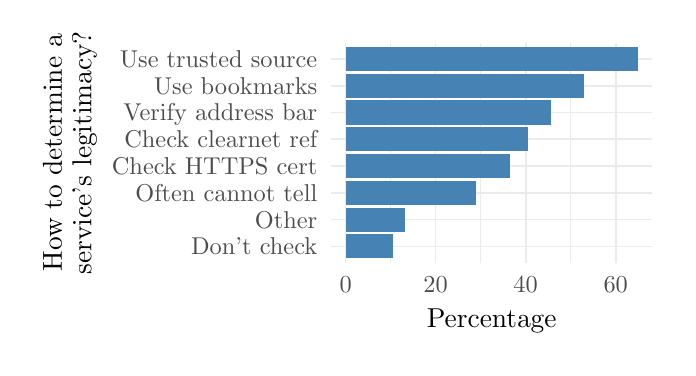
\begin{tikzpicture}[x=1pt,y=1pt]
\definecolor{fillColor}{RGB}{255,255,255}
\path[use as bounding box,fill=fillColor,fill opacity=0.00] (0,0) rectangle (231.26,115.63);
\begin{scope}
\path[clip] (109.60, 30.77) rectangle (225.76,110.13);
\definecolor{drawColor}{gray}{0.92}

\path[draw=drawColor,line width= 0.3pt,line join=round] (131.15, 30.77) --
	(131.15,110.13);

\path[draw=drawColor,line width= 0.3pt,line join=round] (163.68, 30.77) --
	(163.68,110.13);

\path[draw=drawColor,line width= 0.3pt,line join=round] (196.21, 30.77) --
	(196.21,110.13);

\path[draw=drawColor,line width= 0.6pt,line join=round] (109.60, 36.58) --
	(225.76, 36.58);

\path[draw=drawColor,line width= 0.6pt,line join=round] (109.60, 46.26) --
	(225.76, 46.26);

\path[draw=drawColor,line width= 0.6pt,line join=round] (109.60, 55.94) --
	(225.76, 55.94);

\path[draw=drawColor,line width= 0.6pt,line join=round] (109.60, 65.61) --
	(225.76, 65.61);

\path[draw=drawColor,line width= 0.6pt,line join=round] (109.60, 75.29) --
	(225.76, 75.29);

\path[draw=drawColor,line width= 0.6pt,line join=round] (109.60, 84.97) --
	(225.76, 84.97);

\path[draw=drawColor,line width= 0.6pt,line join=round] (109.60, 94.65) --
	(225.76, 94.65);

\path[draw=drawColor,line width= 0.6pt,line join=round] (109.60,104.33) --
	(225.76,104.33);

\path[draw=drawColor,line width= 0.6pt,line join=round] (114.88, 30.77) --
	(114.88,110.13);

\path[draw=drawColor,line width= 0.6pt,line join=round] (147.41, 30.77) --
	(147.41,110.13);

\path[draw=drawColor,line width= 0.6pt,line join=round] (179.95, 30.77) --
	(179.95,110.13);

\path[draw=drawColor,line width= 0.6pt,line join=round] (212.48, 30.77) --
	(212.48,110.13);
\definecolor{fillColor}{RGB}{70,130,180}

\path[fill=fillColor] (114.88, 32.22) rectangle (131.91, 40.93);

\path[fill=fillColor] (114.88, 41.90) rectangle (136.32, 50.61);

\path[fill=fillColor] (114.88, 51.58) rectangle (162.17, 60.29);

\path[fill=fillColor] (114.88, 61.26) rectangle (174.14, 69.97);

\path[fill=fillColor] (114.88, 70.94) rectangle (180.76, 79.65);

\path[fill=fillColor] (114.88, 80.61) rectangle (188.96, 89.32);

\path[fill=fillColor] (114.88, 90.29) rectangle (200.95, 99.00);

\path[fill=fillColor] (114.88, 99.97) rectangle (220.48,108.68);
\end{scope}
\begin{scope}
\path[clip] (  0.00,  0.00) rectangle (231.26,115.63);
\definecolor{drawColor}{gray}{0.30}

\node[text=drawColor,anchor=base east,inner sep=0pt, outer sep=0pt, scale=  0.88] at (104.65, 33.55) {Don't check};

\node[text=drawColor,anchor=base east,inner sep=0pt, outer sep=0pt, scale=  0.88] at (104.65, 43.23) {Other};

\node[text=drawColor,anchor=base east,inner sep=0pt, outer sep=0pt, scale=  0.88] at (104.65, 52.91) {Often cannot tell};

\node[text=drawColor,anchor=base east,inner sep=0pt, outer sep=0pt, scale=  0.88] at (104.65, 62.58) {Check HTTPS cert};

\node[text=drawColor,anchor=base east,inner sep=0pt, outer sep=0pt, scale=  0.88] at (104.65, 72.26) {Check clearnet ref};

\node[text=drawColor,anchor=base east,inner sep=0pt, outer sep=0pt, scale=  0.88] at (104.65, 81.94) {Verify address bar};

\node[text=drawColor,anchor=base east,inner sep=0pt, outer sep=0pt, scale=  0.88] at (104.65, 91.62) {Use bookmarks};

\node[text=drawColor,anchor=base east,inner sep=0pt, outer sep=0pt, scale=  0.88] at (104.65,101.29) {Use trusted source};
\end{scope}
\begin{scope}
\path[clip] (  0.00,  0.00) rectangle (231.26,115.63);
\definecolor{drawColor}{gray}{0.30}

\node[text=drawColor,anchor=base,inner sep=0pt, outer sep=0pt, scale=  0.88] at (114.88, 19.76) {0};

\node[text=drawColor,anchor=base,inner sep=0pt, outer sep=0pt, scale=  0.88] at (147.41, 19.76) {20};

\node[text=drawColor,anchor=base,inner sep=0pt, outer sep=0pt, scale=  0.88] at (179.95, 19.76) {40};

\node[text=drawColor,anchor=base,inner sep=0pt, outer sep=0pt, scale=  0.88] at (212.48, 19.76) {60};
\end{scope}
\begin{scope}
\path[clip] (  0.00,  0.00) rectangle (231.26,115.63);
\definecolor{drawColor}{RGB}{0,0,0}

\node[text=drawColor,anchor=base,inner sep=0pt, outer sep=0pt, scale=  0.99] at (167.68,  7.44) {Percentage};
\end{scope}
\begin{scope}
\path[clip] (  0.00,  0.00) rectangle (231.26,115.63);
\definecolor{drawColor}{RGB}{0,0,0}

\node[text=drawColor,rotate= 90.00,anchor=base,inner sep=0pt, outer sep=0pt, scale=  0.99] at ( 12.32, 70.45) {How to determine a};

\node[text=drawColor,rotate= 90.00,anchor=base,inner sep=0pt, outer sep=0pt, scale=  0.99] at ( 23.01, 70.45) {service's legitimacy?};
\end{scope}
\end{tikzpicture}
